\documentclass[12pt,a4paper]{article}

\usepackage{graphicx}
\usepackage{float}
\usepackage{amsmath}
\usepackage[noend]{algpseudocode}
\usepackage{url}
\graphicspath{ {./images/} }
\renewcommand{\baselinestretch}{1.5}
\everymath{\displaystyle}

\author{Erik-Cristian Seulean}
\title{Dynamic occupancy model for water voles}
\date{\today}

\begin{document}
\newpage
\maketitle
The purpose of this document is to provide an insight into how patch occupancy dynamics can be modelled using Bayesian paradigms in order to assess the prediction that patch occupancy is influenced by area-isolation (Hanski 1998). In other words, it is considered that extinction probabilities are inversely related to patch size and colonization probabilities are positively related to the grade of connectivity of a particular patch to the surrounding patches. In order to test this theory the modelling uses a subset of a dataset available in Sutherland et al. (2014) containing the population of water voles inhabiting in northwest Scotland. For this purpose, we used data available from 114 patches that were surveyed between 2009 and 2014. Every patch was visited between 2 to 4 times every year and the presence of absence of water voles was recorded. Additional to the presence and absence of water voles, each patch contains information about patch length (km.) and a connectivity score that gives insights into how well a particular patch is connected to other patches. The connectivity score is calculated using the dispersion kernel, $e^{-\frac{d_{i,j}}{3}}$ where $d_{i, j}$ represents the distance between patch $i$ and $j$.

In order to test this hypothesis we considered a hierarchical Bayesian model where colonization ($\gamma$) probabilities are modelled as a linear function of connectivity, on the logit scale $log\big(\frac{p}{1-p}\big)$ while extinction is modelled as a linear function of patch length, on the logit scale as well. Both extinction and colonization are modelled on the logit scale to ensure that the domain is $[0, 1]$ and obey the laws of probability. Given that no initial occupancy is known (as it would be the case in a reintroduction project) we will consider an uninformative prior for the initial occupancy $\psi_{1} \sim \mathcal{U}(0, 1)$ while alternative Beta priors could be considered if we have an intuition on where the higher mass percentage could be distributed. To admit to the fact that detection probabilities are not constant during the period of the study, the model considers the detection probabilities normally distributed with unknown mean and variance, on the logit scale. To address the lack of knowledge of the mean and variance, we consider uninformative priors $\mu \sim \mathcal{U}(-10, 10)$, $\sigma \sim \mathcal{U}(0, 5)$. For the two linear models $logit(\epsilon_{i,t}) = a_{0} + a_{1}\mathcal{L}_{i}$ and $logit(\gamma_{i, t}) = b_{0} + b_{1}\mathcal{C}_{i}$, with $L_{i}$ the length and $C_{i}$ the connectivity of the $i^{th}$ we will consider Normal distributed priors for the slope and intercept of the two linear models. $\mathcal{N}(\mu=0, \sigma^{2}=10)$.

The model considers the occupancy state $z_{i, t}$ of patch $i$ at time $t$ as a function of the patch state at the previous timestamp. In other words, a patch that is occupied at time $t-1$ will be occupied at time $t$ if it does not go extinct or alternatively if it's not occupied at $t-1$ will be occupied at time $t$ if it's colonized. $$z_{i, t} = (1 - z_{i, t-1})\gamma_{i, t-1} + z_{i, t-1}(1-\epsilon_{i, t-1})$$. 

The observations are considered to be drawn from a Binomial distribution, with probability of success equal to the probability of detection if the site is occupied or 0 otherwise, and the number of trials represent the number of visits done at that particular site in that year. Furthermore, the analysis included additional intermediary calculations to facilitate construction of tests that increase the confidence in the model.

In order to fit and simulate from this model we used a MCMC simulation using the BUGS paradigm in R where 3 chains performed 10000 iterations out of which we discarded 3000 for burn-in. To account for autocorrelation in the samples, we applied thinning, storing every 6th iteration from every chain. This lead to a number of effective samples between 400 and 3500. The assessment of convergence was done using trace plots for the parameter of interest, additional to checks using the Gelman-Rubin diagnostic. In this case, $\hat{R}$ shows a value smaller than 1.1, proving that convergence is achieved. (see appendix for randomly selected trace plots). The density plots for $\gamma$, $\epsilon$ and $p$ are further evidence that convergence is achieved, given that all chains peak in the same area and there are no disagreements that lead to multimodal posterior distributions. In order to check how well the sample data fits the distribution, goodness of fit tests were performed. The null hypothesis for this model is that there is no significant difference between the observed and simulated data. With Bayesian p-value 0.54 we have no reason to reject the null hypothesis, concluding that the model is adequate. 

\begin{figure} [H]
    \begin{center}
        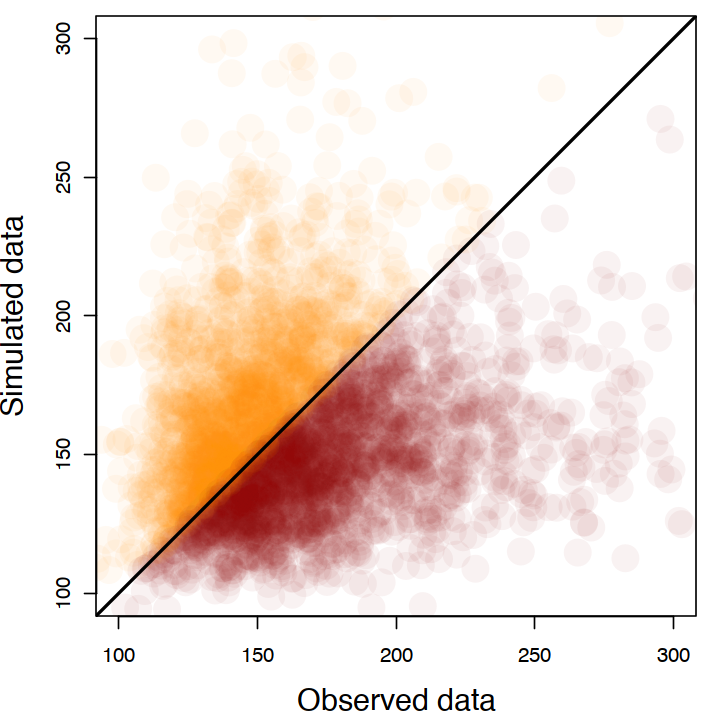
\includegraphics[scale=0.6, width=6cm]{chisq.png}
        \label{fig:sampledvsdata}
        \caption{Observed proportion 0.54}
    \end{center}
\end{figure}

Given the details above, we can draw conclusions about the model and the population itself. First, extinction probabilities are indeed inverse related to patch size (in this case length). As patch size increases, we expect the extinction probabilities to decrease, and the simulation shows a negative correlation of -0.8 between patch length and extinction probability. Furthermore, the colonization probability is indeed increasing with the connectivity, the simulation providing evidence of a very high correlation of 0.87. 

\begin{figure} [H]
    \centering
    \textbf{Extinction and colonization probabilities}\par\medskip
    \begin{minipage}{.5\textwidth}
      \centering
      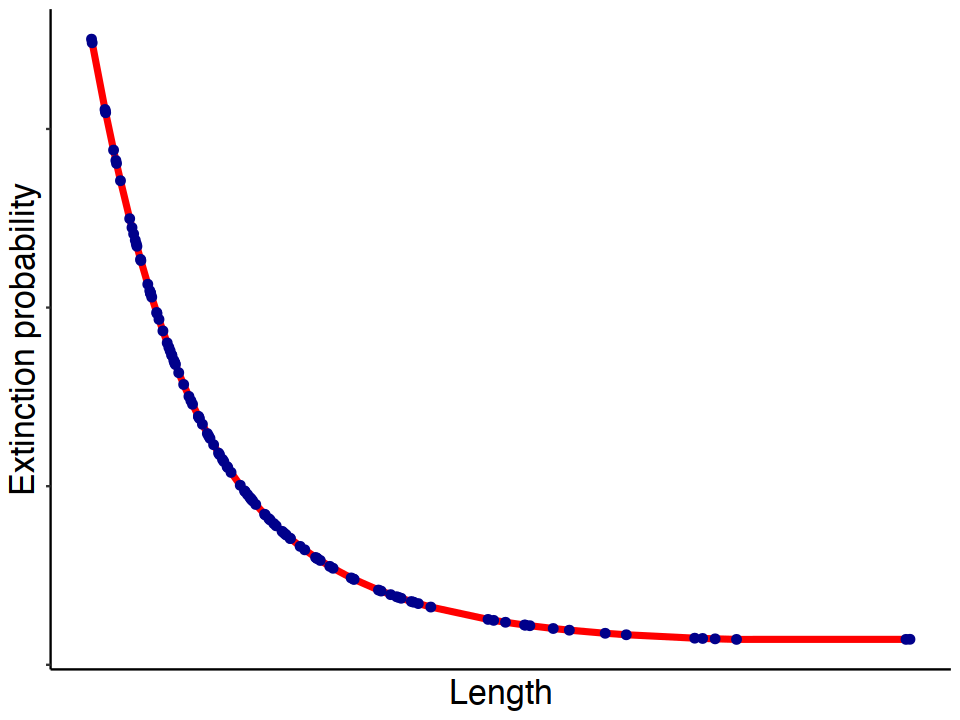
\includegraphics[width=0.8\linewidth]{extinction_by_length.png}
      \caption{Extinction}
      \label{fig:Extinction by patch length}
    \end{minipage}%
    \begin{minipage}{.5\textwidth}
      \centering
      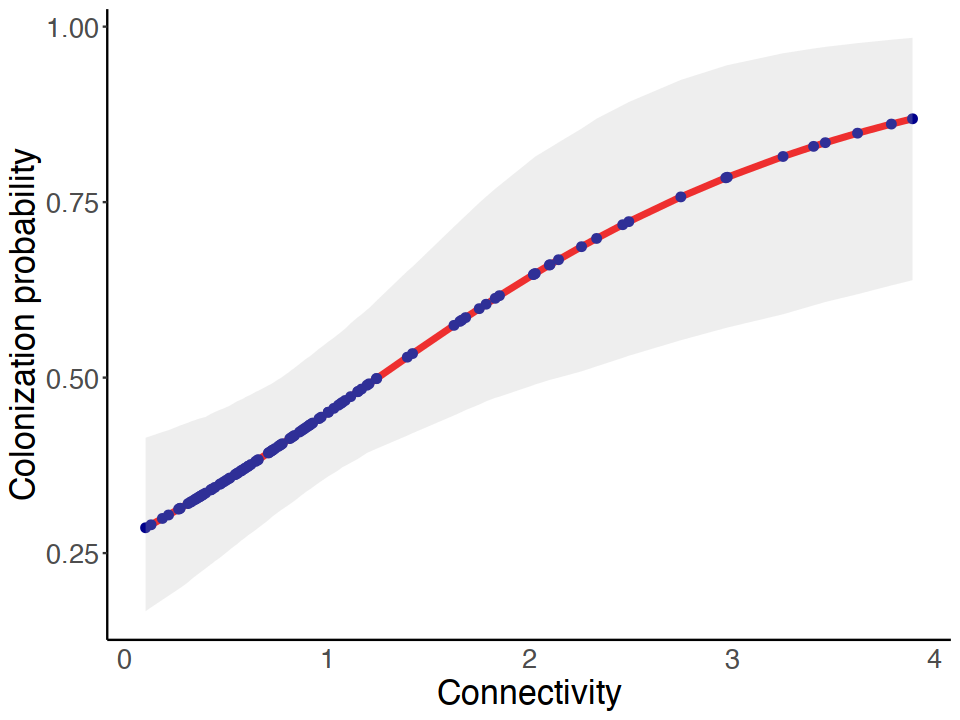
\includegraphics[width=0.8\linewidth]{colonization_by_connectivity.png}
      \caption{Colonization}
      \label{fig:Colonization by connectivity}
    \end{minipage}
\end{figure}

The above statements agree with the fact that patch occupancy dynamics emerge according to the area-isolation paradigm as mentioned in Hanski 1998, at least in the case of water voles inhabitating northwest of Scotland.

Besides checking the theories behind patch occupancy dynamics, the model also offers insights into the percentage of patches that are occupied. During the surveyed period, we expect that the percentage of sites occupied grow from $63\%$ (($54\%$ - $74\%$) Bayesian credible interval) in 2009 to around $90\%$ (($77\%$ - $96\%$) Bayesian credible interval) in 2014. A five years projection estimates that patch occupancy will continue to be over $90\%$ between 2012 and 2017.
\maketitle

\end{document}\models